                \begin{figure}[ht]
                        \centerline{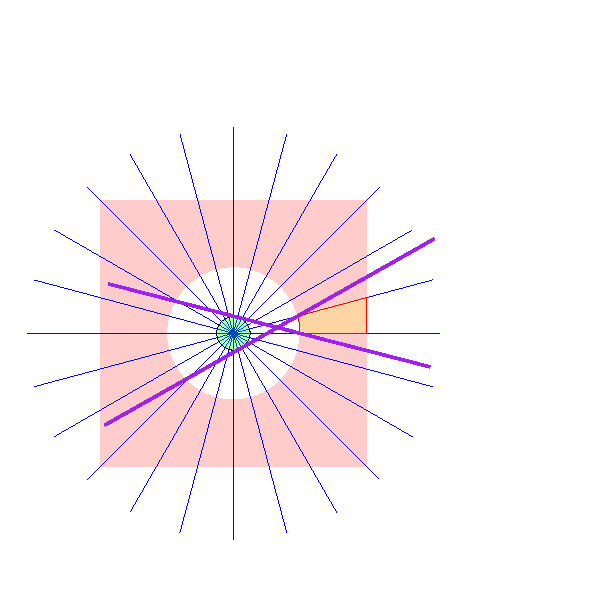
\includegraphics{../figs/partition}}
                        \caption{An illustration of refining the pairs in a \SSPD into
                                pairs contained in opposite parts of an
                                $\eps$-double-wedge. $\PSX$ is contained in the green square
                                $\square$, while $\PSY$ is contained in the red square, and the
                                white gap between them is a result of the separation
                                property. The set of cones with the apex at the center of
                                $\square$ gives us the desired partition as demonstrated by the
                                purple double-wedge. }
                        \figlab{partition}
                \end{figure}
        
                By using \lemref{chop:easy}, we can assume that $\WS$ is (say)
                $(10/\eps)$-separated. For each pair
                $\Pair = \{ \PSX, \PSY \} \in \WS$, assume that
                $\diameterX{\PSX} < \diameterX{\PSY}$. Now, the algorithm scans
                the pairs of $\WS$ and performs the following procedure for each
                one. Let $\square$ be the smallest axis-parallel square containing
                $\PSX$, centered at point $\origin$. Partition the plane around
                $\origin$, by drawing $\Of(1/\eps)$ lines intersecting $\origin$
                with the angle between any two consecutive lines being at most
                (say) $\eps/4$, see \figref{partition}. This partitions the plane
                into a set of cones $\ConeSet$. For a cone $\cone \in \ConeSet$,
                we show that there exists an $\eps$-double-wedge that contains
                $\PSX$ in one side, and $\PSY \cap \cone$ in the other.
                
                To see that, take the double-wedge formed by the cross tangents
                between $\CHX{\PSX}$ and $\CHX{\PSY \cap \cone}$, where
                $\CHX{\PSX}$ denotes the convex-hull of $\PSX$. Assume w.l.o.g
                that $\square$ has side length 1, and let $\coneB$ be a cone of
                angle $\eps / 4$ with apex $\origin$, whose angular bisector is a
                horizontal ray in the positive direction of the $x$ axis. See
                figure \figref{double-wedge} for an illustration.
                
                \begin{figure}[h]
                        \phantom{}\hfill%
                        \includegraphics[page=2,
                        width=0.48\linewidth]{../figs/double_wedge}%
                        \hfill%
                        \includegraphics[page=3,
                        width=0.48\linewidth]{../figs/double_wedge}%
                        \hfill%
                        \phantom{}%
                        \caption{An illustration of the proof for \lemref{refine:d:w}}
                        \figlab{double-wedge}
                \end{figure}
                
                We would like to find a vertical segment $\seg$ such that all
                points of $\PSY$ lie to its right, with one endpoint on the upper
                line of $\coneB$, and the other on the lower line of
                $\coneB$. Using the segments' height and distance from the right
                side of $\square$ we will be able to get a bound on the angle of
                the cross tangents. We first find a segment $\seg$ with all points
                of $\PSY$ to its right. A trivial bound on that distance is given
                by the segment from, say, the lower left corner of $\square$,
                denoted $\pa$, of length $10/\eps$ with its right endpoint on the
                upper line of $\coneB$, denote this point by $\pb$. We know that
                all points of $\PSY$ lie to the right of $\pb$ due to the
                $10/\eps$ separation property of the \SSPD. The segment $\pa\pb$
                creates an angle $\leq\pi/4$ with the $x$-axis (by the choice of
                the angle of $\coneB$).  We therefore get that the $x$-coordinate
                difference between $\square$ and $\pb$ is at most
                $10/\eps\cdot \cos\frac{\pi}{4}-1\leq 7/\eps-1\leq 6/\eps$. So,
                let $\seg'$ be a vertical segment between the upper and lower rays
                of $\coneB$, with $x$-coordinate distance of $6/\eps-\frac{1}{2}$
                from $\square$ (in order to make calculations easier). We get that
                $s'$ is of length $2\cdot \frac{6}{\eps}\tan
                \frac{\eps}{8}$. Finally, we take $\seg$ to be a vertical segment
                of length $\frac{12}{\eps}\tan \frac{\eps}{8}$, with its center on
                the $x$-axis at a distance of $5/\eps+\frac{1}{2}$ away from
                $\origin$. The angle of the $x$-axis and the segment between the
                lower end of the right side of $\square$ and the upper end of
                $\seg$ is now given by:
                
                \begin{equation*}
                        \arctan
                        \pth{\frac{\frac{6}{\eps}
                                        \tan\frac{\eps}{8}+\frac{1}{2}}{\frac{5}{\eps}}
                        }%
                        =%
                        \arctan \pth{ \frac{6}{5}\tan\frac{\eps}{8}+\frac{\eps}{10} }%
                        \leq%
                        \eps%
                \end{equation*}
